% Section name and highlighted ToC
\renewcommand{\sectiontitle}{Minimum Makespan Scheduling}
\section{\sectiontitle}
\customToC{currentsection,hideothersubsections}{}

\renewcommand{\subsectiontitle}{Descripción del problema}
\subsection{\subsectiontitle}

\begin{frame}{\subsectiontitle}
    \begin{itemize}
        \item Sean \(J_{1}, J_{2}, \dotsc, J_{n}\) trabajos cuyos tiempos de procesamiento son \(p_{1}, p_{2}, \dotsc, p_{n}\)
        respectivamente y un entero positivo \(m\) \textit{(el número de máquinas)}, encontrar un asignación de los 
        \(n\) trabajos a las \(m\) máquinas tal que el tiempo que se tardan en completar éstos trabajos en las máquinas
        \textbf{(que es llamado \textit{makespan})} es mínimo.
    \end{itemize}
\end{frame}

\renewcommand{\subsectiontitle}{Entendiendo el enunciado}
\subsection{\subsectiontitle}

\begin{frame}{\subsectiontitle}
    \begin{itemize}
    \item Las \(m\) máquinas son idénticas entre sí, es decir, tienen el mismo poder de cómputo.
    \item Los trabajos no pueden ser divididos entre las máquinas.
    \item Definimos al conjunto \(A_{j}\) como el conjunto de índices de los trabajos asignados a la máquina \(j\) con \(1 \leq j \leq m\).
\end{itemize}
\end{frame}

\begin{frame}{\subsectiontitle}
    \begin{itemize}
        \item Definimos a \(T_{j}\) como \(\displaystyle\sum_{i \in A_{j}} p_{i}\), notemos que \(T_{j}\) el tiempo total 
        de procesamiento que toma ejecutar todos los trabajos asignados a la máquina \(j\).
        \item Lo que debemos de encontrar es una asignación de los trabajos a las máquinas de tal manera que el \textbf{makespan}
        sea mínimo, es decir buscamos minimizar \(\mathbf{max} \ T_{j}\), para toda \(1 \leq j \leq m\).
    \end{itemize}
\end{frame}

\renewcommand{\subsectiontitle}{Algoritmo 2 aproximado}
\subsection{\subsectiontitle}

\begin{frame}{\subsectiontitle}
    Sean \(J_{1}, J_{2}, \dotsc, J_{n}\) trabajos
    \begin{itemize}
        \item Ordenamos los \(n\) trabajos de manera arbitraria. Es decir, los trabajos después de ordenarlos serán:
        \[
            J_{\sigma\left(1\right)}, J_{\sigma\left(2\right)}, \dotsc, J_{\sigma\left(n\right)}
        \]
        donde \(\sigma\) es una permutación del conjunto \(\{1, 2, \dotsc, n\}\).
        \item Ir ejecutando los \(n\) trabajos en las \(m\) máquinas en el nuevo orden de la siguiente manera:
        \begin{itemize}
            \item Sea \(J_{\sigma\left(i\right)}\) el siguiente trabajo a ejecutar con el orden obtenido en el paso anterior,
            \(J_{\sigma\left(i\right)}\) se ejecutará en el procesador que tenga la menor carga de trabajo en ese momento.
        \end{itemize}
    \end{itemize}
\end{frame}

\renewcommand{\subsectiontitle}{Cota inferior}
\subsection{\subsectiontitle}

\begin{frame}{\subsectiontitle}
    El algoritmo descrito anteriormente fue diseñado tomando en cuenta las siguientes \textbf{cotas inferiores} en la 
    solución óptima, \(\mathbf{OPT}\).
    \begin{itemize}
        \item El tiempo de procesamiento promedio de todas las máquinas el cuál es: \(\frac{1}{m}\displaystyle\sum_{i=1}^{n}p_{i}\).
        \item El tiempo de procesamiento más largo correspondiente a algún trabajo, es decir: \(\mathbf{max}\{p_{i}\}\).
    \end{itemize}
    Así sea \(\mathbf{LB}\) la cota inferior que considera ambos casos, y la definimos como sigue:
    \[
        \mathbf{LB} = \mathbf{max}\left \{ \frac{1}{m}\displaystyle\sum_{i=1}^{n}p_{i}, \mathbf{max}\{p_{i}\} \right \}
    \]
\end{frame}

\renewcommand{\subsectiontitle}{Teorema}
\subsection{\subsectiontitle}

\begin{frame}{\subsectiontitle}
    \begin{itemize}
        \item El algoritmo descrito anteriormente es un \textbf{algoritmo 2 aproximado}.
    \end{itemize}
\end{frame}

\renewcommand{\subsectiontitle}{Demostración}
\subsection{\subsectiontitle}

\begin{frame}{\subsectiontitle}
    \begin{itemize}
        \item Sea \(T\) el \textbf{makespan óptimo}, entonces notamos que \(T\) cumple con las siguientes desigualdades:
        \begin{align*}
            T &\geq \mathbf{max}\{p_{i}\} \\
            T &\geq \frac{1}{m} \sum_{j=1}^{m} T_{j} = \frac{1}{m} \sum_{i=1}^{n} p_{i}
        \end{align*}
        \item Es muy sencillo argumentar el porqué ambas desigualdades son verdaderas.
    \end{itemize}
\end{frame}

\begin{frame}{\subsectiontitle}
    Veamos \(T \geq \mathbf{max}\{p_{i}\}\)
    \begin{itemize}
        \item Por definición \(T = \mathbf{max} \ T_{j}\), para alguna \(1 \leq j \leq m\).
        \item De nuevo por definición tenemos que \(T = \mathbf{max} \displaystyle\sum_{i \in A_{j}} p_{i}\) para alguna \(1 \leq j \leq m\).
    \end{itemize}
\end{frame}

\begin{frame}{\subsectiontitle}
    Tenemos dos casos:
    \begin{itemize}
        \item \(\mathbf{max}\{p_{i}\}\) forma parte de los sumandos de \(T\), así puede ocurrir lo siguiente:
        \begin{itemize}
            \item \(T\) solamente tiene un sumando, así se tiene que se cumple \(T \geq \mathbf{max}\{p_{i}\}\), ya que en particular \(T = \mathbf{max}\{p_{i}\}\).
            \item \(T\) tiene más sumandos además de \(\mathbf{max}\{p_{i}\}\) así se tiene que se cumple \(T \geq \mathbf{max}\{p_{i}\}\), ya que en particular \(T > \mathbf{max}\{p_{i}\}\)
        \end{itemize}
        \item \(\mathbf{max}\{p_{i}\}\) no forma parte de los sumandos de \(T\), así \(p_{i}\) forma parte de alguna \(T_{k}\) tal que \(T \geq T_{k}\), así obtenemos que 
        \(T \geq \mathbf{max}\{p_{i}\}\).
    \end{itemize}
\end{frame}

\begin{frame}{\subsectiontitle}
    Veamos \(T \geq \frac{1}{m} \sum_{j}^{m} T_{j}\)
    \begin{itemize}
        \item Es inmediata ésta desigualdad.
    \end{itemize}
\end{frame}
\begin{frame}{\subsectiontitle}
    \begin{itemize}
        \item Sea \(M_{i}\) la última máquina que completa los trabajos que se le asignaron a través del algoritmo y sea \(j\) el índice del último trabajo 
        ejecutado sobre \(M_{i}\). 
        \item Entonces por construcción el máximo tiempo de procesamiento está en \(M_{i}\), es decir, \(T_{i} \geq T_{k}\) para toda \(1 \leq k \leq m\) con \(k \neq i\). 
    \end{itemize}
\end{frame}
\begin{frame}{\subsectiontitle}
    \begin{itemize}
        \item Se deduce fácilmente que la máquina \(M_{i}\) tiene la menor carga de trabajo al momento de asignar al trabajo \(J_{j}\) a ejecutarse en dicha máquina \textit{(definición del algoritmo)}. 
        \item Consecuentemente la máquina \(M_i\) tiene un tiempo de procesamiento más pequeño que el promedio.
    \end{itemize}
\end{frame}
\begin{frame}{\subsectiontitle}
    \begin{itemize}
        \item Lo que hemos dicho es que:
            \begin{align*}
                T_{i} - p_{j} &\leq \frac{1}{m}\sum_{k=1}^{n}p_{k}
            \end{align*}
        \item \(T_{i} - p_{j}\) es el momento en el cuál se asignó la ejecución del trabajo \(J_{j}\) en la máquina \(M_{i}\).
        \item Es trivial ver que:
        \begin{align*}
            p_{j} &\leq \mathbf{max}\{p_{k}\}
        \end{align*}
    \end{itemize}
\end{frame}

\begin{frame}{\subsectiontitle}
    \begin{itemize}
        \item Así
        \begin{align*}
            T_{i} &= \left(T_{i} - p_{j} \right) + p_{j} \\
                  &\leq \frac{1}{m}\sum_{k=1}^{n}p_{k} + \mathbf{max}\{p_{k}\} \\
                  &\leq T + T = 2 \cdot T
        \end{align*}
        \item Por lo tanto el algoritmo es un \textbf{algoritmo \(2\) aproximado}.
    \end{itemize}
\end{frame}

\begin{frame}{\subsectiontitle}
    \begin{figure}[H]
        \centering
        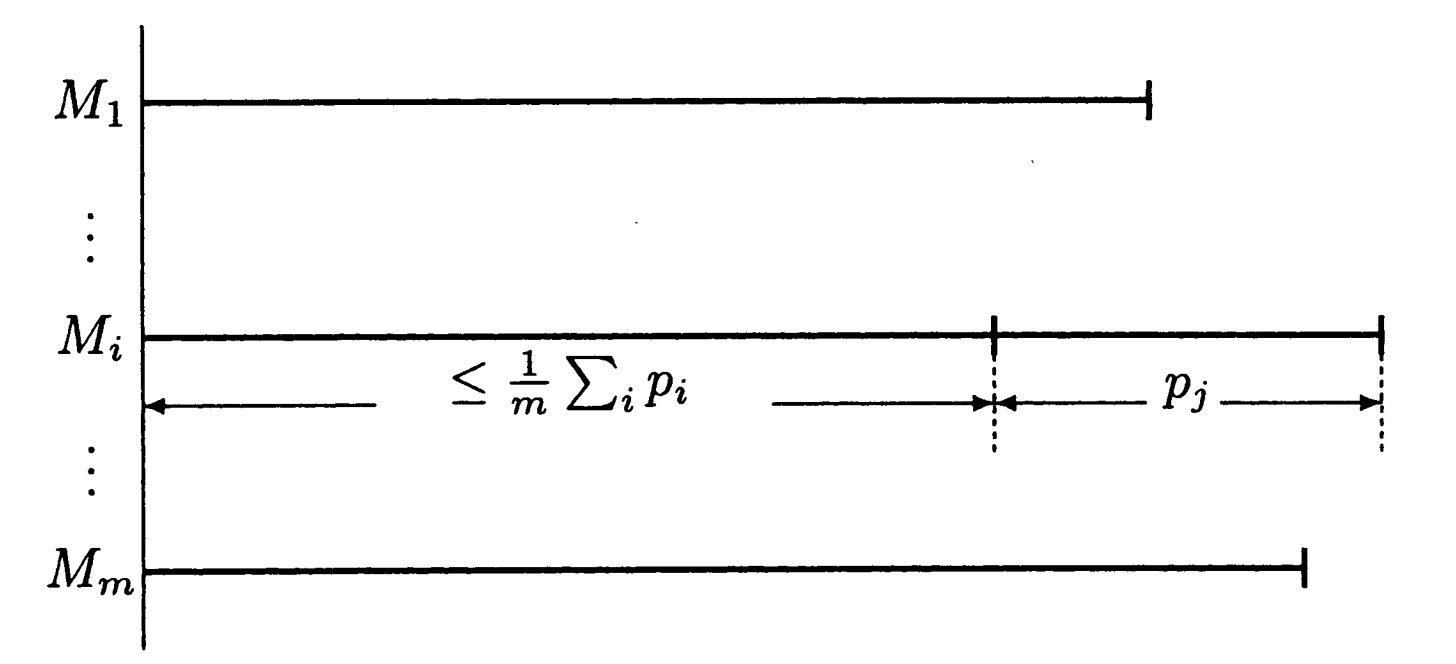
\includegraphics[scale=0.25]{imgs/MMS/img1_cc.jpg}
    \end{figure}
\end{frame}

\renewcommand{\subsectiontitle}{Ejemplo}
\subsection{\subsectiontitle}

\begin{frame}{\subsectiontitle}
    \begin{itemize}
    \item \(n = m^2 + 1\)
    \item Los trabajos son:
    \[
        J_{1}, J_{2}, \dotsc, J_{m^2 - 1}, J_{m^2}, J_{m^2 + 1}
    \]
    \item \(p_{i} = 1\) para toda \(i \in \{1, 2, \dotsc, m^2-1, m^2\}\)
    \item \(p_{m^2 + 1} = m\) 
    \item El \textbf{makespan óptimo} es \(m + 1\).
    \item El \textbf{makespan obtenido por el algoritmo} es \(2m\).
\end{itemize}
\end{frame}

\begin{frame}{\subsectiontitle}
    \textbf{Makespan óptimo}
    \begin{itemize}
        \item Notemos que el mejor de los casos sería que una máquina ejecute el trabajo \(J_{m^2 + 1}\) con un tiempo de duración de \(m\) unidades de tiempo.
        \item Así los otros \(m^2\) trabajos restantes tienen
        un tiempo de duración de una unidad de tiempo.
        \item Mientras que alguna máquina \(i\) con \(1 \leq i \leq m\) ejecuta el trabajo \(J_{m^2+1}\) las restantes \(m-1\) máquinas ejecutan cada una un trabajo con un tiempo de duración de una unidad de tiempo durante \(m\) unidades de tiempo \textit{(que es lo que dura el trabajo} \(J_{m^2+1}\) \textit{)}.
    \end{itemize}
\end{frame}

\begin{frame}{\subsectiontitle}
    \textbf{Makespan óptimo}
    \begin{itemize}
        \item Al finalizar el tiempo \(m\) los trabajos que se han ejecutados están dados por la siguiente expresión:
        \begin{align*}
            m(m-1) + 1 = m^2 - m + 1
        \end{align*}
        \item A los trabajos que nos faltan por ejecutar están dados por la expresión:
        \begin{align*}
            m^2 + 1 - ( m^2 - m + 1) &= m^2 + 1 - m^2 + m - 1 \\
            m^2 - m^2 + 1 - 1 + m &= m
        \end{align*}
        \item En éste momento contamos con \(m\) máquinas disponibles para los \(m\) trabajos así en todos los casos tenemos que \(T_{i} = m + 1\) para toda \(1 \leq i \leq m\). Por lo tanto el \textbf{makespan óptimo} es \(m + 1\).
    \end{itemize}
\end{frame}

\begin{frame}{\subsectiontitle}
    \textbf{Makespan dado por el algoritmo}
    \begin{itemize}
        \item Notemos que en el peor de los casos el algoritmo nos proporciona el siguiente orden para los trabajos:
        \[
            J_{\sigma\left(1\right)}, J_{\sigma\left(2\right)}, \dotsc, J_{\sigma\left(m^2\right)}, J_{\sigma\left(m^2+1\right)}
        \]
        con \(\sigma\) una permutación del conjunto \(\{1, 2, \dotsc, m^2, m^2 + 1\}\) y \(\sigma\left(m^2+1\right) = m^2+1\).
        \item Dado lo anterior, el último trabajo en ejecutarse es el trabajo \(J_{m^2+1}\) cuyo tiempo de duración es de \(m\) unidades de tiempo.
    \end{itemize}
\end{frame}

\begin{frame}{\subsectiontitle}
    \textbf{Makespan dado por el algoritmo}
    \begin{itemize}
        \item Por la descripción del algoritmo en las primeras \(m\) unidades de tiempo las \(m\) máquinas ejecutan en cada unidad de tiempo un trabajo cuya duración es de una unidad de tiempo así, los trabajos ejecutados hasta el tiempo \(m\) están dados por la expresión:
        \[
            m(m) = m^2  
        \]
        \item Al finalizar el tiempo \(m\), alguna de las \(m\) máquinas ejecutará el trabajo \(J_{m^2+1}\) dándonos así que el \textbf{makespan} dado por el algoritmo es de \(2m\).
    \end{itemize}
\end{frame}

\renewcommand{\subsectiontitle}{¿Es un PTAS?}
\subsection{\subsectiontitle}

\begin{frame}{\subsectiontitle}
    \begin{itemize}
        \item No es un \textbf{PTAS}\textit{(Polynomial Time Approximation Scheme)}.
    \end{itemize}
\end{frame}

%\renewcommand{\subsectiontitle}{PTAS}
%\subsection{\subsectiontitle}

%\begin{frame}{\subsectiontitle}
%    \begin{itemize}
%        \item
%    \end{itemize}
%\end{frame}

\renewcommand{\subsectiontitle}{Bin Packing}
\subsection{\subsectiontitle}

\begin{frame}{\subsectiontitle}
    \textbf{Descripción del problema}
    \begin{itemize}
        \item Dados \(n\) objetos con tamaños \(a_{1}, a_{2}, \dotsc, a_{n}\) tal que \(0 < a_{i} \leq 1\) para todo \(1 \leq i \leq n\).
        \item Encontrar un empaquetamiento en contenedores de tamaño \(1\) tal que el número de contenedores usado es el mínimo.
    \end{itemize}
\end{frame}

\begin{frame}{\subsectiontitle}
    \begin{figure}[H]
        \centering
        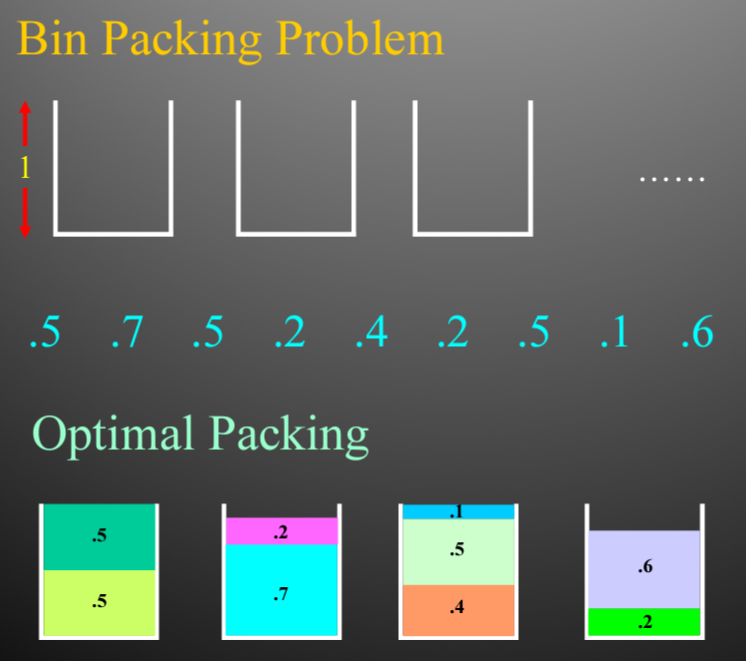
\includegraphics[scale=0.3]{imgs/MMS/img2_cc.jpg}
    \end{figure}
\end{frame}

\begin{frame}{\subsectiontitle}
    \textbf{Relación con minimum makespan scheduling}
    \begin{itemize}
        \item El problema \textbf{minimum makespan scheduling} está íntimamente relacionado con el problema de \textbf{bin packing} ya que existe una caledarización \textit{(scheduling)} con un \textbf{makespan} de tiempo \(t\) sí y solamente sí \(n\) objetos de tamaños 
        \(p_{1}, p_{2}, \dotsc, p_{n}\) pueden ser empacados en \(m\) contenedores de tamaño \(t\) cada uno. 
        \item Es decir, existe una 
        reducción del problema \textbf{minimum makespan scheduling} al problema de \textbf{bin packing}, ya que:
        \begin{itemize}
            \item De \(n\) trabajos pasamos a \(n\) objetos.
            \item De los tiempos de duración \(p_{1}, p_{2}, \dotsc, p_{n}\) correspondientes a los \(n\) trabajos pasamos a los 
            tamaños \(p_{1}, p_{2}, \dotsc, p_{n}\) de los \(n\) objetos.
            \item De \(m\) máquinas para ejecutar los trabajos pasamos a \(m\) contenedores para guardar los objetos.
            \item Del \textbf{makespan} el cual es \(t\) pasamos a que cada contenedor tenga tamaño \(t\).
        \end{itemize}
            \end{itemize}
\end{frame}

\renewcommand{\subsectiontitle}{Descripción del esquema de aproximación}
\subsection{\subsectiontitle}

\begin{frame}{\subsectiontitle}
    \textbf{Notación}
    \begin{itemize}
    \item Denotaremos al conjunto de los tamaños de los \(n\) objetos, los cuales son \(p_{1}, p_{2}, \dotsc, p_{n}\) 
    con la letra \(I\).
    \item \(\mathbf{bins}\left(I,t\right)\) es el mínimo número de contenedores de tamaño \(t\) que se necesitan 
    para empacar los \(n\) objetos.
    \item El \textbf{makespan} mínimo está dado por \(\mathbf{min}\{ \ t \ : \ \mathbf{bins}\left(I, t\right) \ \leq \ m\}\)
\end{itemize}
\end{frame}

\begin{frame}{\subsectiontitle}
    \begin{itemize}
    \item Hacemos la observación de que \(LB\) es una cota inferior y \(2 \cdot LB\) es una cota superior del \textbf{makespan} mínimo.
    \item Lo que se hará es determinar el \textbf{makespan} mínimo por búsqueda binaria en el intervalo \([LB, 2 \cdot LB]\). 
    \item El problema se puede resolver en tiempo polinomial sí el conjunto de los tamaños de los objetos es finito y su cardinalidad es fija.
\end{itemize}
\end{frame}

\begin{frame}{\subsectiontitle}
    \textbf{Bin packing con un número fijo de tamaños de los objetos.}
    \begin{itemize}
    \item Sea \(k\) el número fijo que denota los distintos tamaños de los objetos y supondremos que los contenedores tiene capacidad de \(1\).
    \item Ordenamos el tamaño de los objetos.
    \item Ahora un ejemplar genérico del problema de \textbf{bin packing} puede ser descrito de la siguiente manera:
    \begin{itemize}
        \item Una \(k-\)tupla definida como \(\left(i_{1}, i_{2}, \dotsc, i_{k}\right)\) donde cada \(i_{j}\) con \(1 \leq j \leq k\) especifica
        el número de objetos que tienen un tamaño que está en el conjunto \(I\), es decir, \(\left(i_{1}, i_{2}, \dotsc, i_{k}\right)\) especifica
        el número de de objetos de cada tamaño.
    \end{itemize}
    \item \(\mathbf{BINS}\left(i_{1}, i_{2}, \dotsc, i_{k}\right)\) denota el número mínimo de contenedores que son necesitados para empacar éstos objetos.
\end{itemize}
\end{frame}

\begin{frame}{\subsectiontitle}
    \textbf{Algoritmo de programación dinámica}
    \begin{itemize}
        \item Sea \(\left(n_{1}, n_{2}, \dotsc, n_{k}\right)\) un ejemplar del problema de \textbf{bin packing con número fijo de tamaños de los objetos} tal que 
        \(\displaystyle\sum_{i=1}^{k}n_{i} = n\)
        \item Calcularemos el conjunto \(\mathcal{Q}\) cuyos elementos serán todas las \(k-\)tuplas 
        \(\left(q_{1}, q_{2}, \dotsc, q_{k}\right)\) tales que:
        \begin{itemize}
            \item \(\mathbf{BINS}\left(q_{1}, q_{2}, \dotsc, q_{k}\right) = 1\)
            \item y además
                    \begin{align*}
                        &0 \leq q_{i} \leq n_{i} \\
                        &1 \leq i \leq k
                    \end{align*}
        \end{itemize}
    \end{itemize}
\end{frame}

\begin{frame}{\subsectiontitle}
    \begin{itemize}
        \item \(\mathcal{Q}\) contiene a lo más \(O\left(n^k\right)\) elementos, ésto es muy sencillo de ver.
        \item Denotamos como \(w_{i}\) al peso de cada uno de los \(n_{i}\) objetos.
        \item Así el peso total de los \(n_{i}\) objetos está dado por \(w_{i} \cdot n_{i}\) para toda \(1 \leq i \leq k\).
        \item Sí ocurre que:
        \[
            \left(\sum_{i = 1}^{n}  w_{i} \cdot n_{i}\right) \leq 1
        \]
        \item Entonces cualquier \(k-\)tupla \(\left(q_{1}, q_{2}, \dotsc, q_{k}\right)\) tales que:
        \begin{align*}
            &0 \leq q_{i} \leq n_{i} \\
            &1 \leq i \leq k
        \end{align*}
        cumplirá que \(\mathbf{BINS}\left(q_{1}, q_{2}, \dotsc, q_{k}\right) = 1\) 
        \item Así el número de tuplas está dado por:
        \[
            (n_{1} + 1) \cdot (n_{2} + 1) \dotsm  (n_{k-1} + 1) \cdot (n_{k} + 1)
        \]
    \end{itemize}
\end{frame}

\begin{frame}{\subsectiontitle}
    \begin{itemize}
        \item Es \(n_{i} + 1\) para toda \(1 \leq i \leq k\) ya que tenemos que contar la opción de poner el número \(0\).
        \item Tenemos que 
        \[
            n_{i} \leq n
        \]
        para toda \(1 \leq i \leq k\).
        \item Trivialmente tenemos que:
        \[
            n_{i} + 1 \leq n + 1
        \]
        para toda \(1 \leq i \leq k\).
        \item Así 
        \begin{align*}
            (n_{1} + 1) \cdot (n_{2} + 1) \dotsm (n_{k-1} + 1) \cdot (n_{k} + 1) &\leq (n + 1) \cdot (n + 1) \dotsm (n + 1) \cdot (n + 1) \\
            (n_{1} + 1) \cdot (n_{2} + 1) \dotsm (n_{k-1} + 1) \cdot (n_{k} + 1) &\leq (n + 1)^{k}
        \end{align*}
        de ahí la complejidad en tiempo.
    \end{itemize}

\end{frame}

\begin{frame}{\subsectiontitle}
    \begin{itemize}
        \item Ahora calcular todas las \(\mathbf{BINS}\left(i_{1}, i_{2}, \dotsc, i_{k}\right)\) para cada \(k-\)tupla
        \(\left(i_{1}, i_{2}, \dotsc, i_{k}\right) \in \mathcal{Q}'\) 
        \item El conjunto \(\mathcal{Q}'\) está 
        definido como sigue:
        \[
            \mathcal{Q}' = \{0, \dotsc, n_{1}\} \times \{0, \dotsm, n_{2}\}  \times \dotsm \times \{0, \dotsc, n_{k}\}  
        \]
        \item Hacemos la observación de que \(\mathbf{BINS}\left(q\right) = 1\) para todo \(q \in \mathcal{Q}\).
    \end{itemize}
\end{frame}

\begin{frame}{\subsectiontitle}
    \begin{itemize}
        \item El cálculo se hará de manera recursiva como sigue:
        \[
            \mathbf{BINS}\left(i_{1}, i_{2}, \dotsc, i_{k}\right) = 1 + \min_{q \in \mathcal{Q}} \ \mathbf{BINS}\left(i_{1} - q_{1}, i_{2} - q_{2}, \dotsc, i_{k} - q_{k}\right)
        \]
        \item Calcular cada \(\mathbf{BINS}\left(i_{1}, i_{2}, \dotsc, i_{k}\right)\) nos toma tiempo \(O\left(n^{k}\right)\) ya que de nuevo en el peor de los casos el conjunto \(\mathcal{Q}\) tiene \(O\left(n^{k}\right)\) elementos.
        \item Por lo tanto calcular todos los \(\mathbf{BINS}\left(i_{1}, i_{2}, \dotsc, i_{k}\right)\) nos toma tiempo \(O\left(n^{2k}\right)\).
        \item Al calcular todos los \(\mathbf{BINS}\left(i_{1}, i_{2}, \dotsc, i_{k}\right)\), podemos determinar \(\mathbf{BINS}\left(n_{1}, n_{2}, \dotsc, n_{k}\right)\).
    \end{itemize}
\end{frame}

\begin{frame}{\subsectiontitle}
    \begin{itemize}
        \item Podemos aceptar algunos error al calcular \textbf{minimum makespan scheduling}. Sólo hay dos formas de generar un error las cuales son:
        \begin{itemize}
            \item Redondear los tamaños de los objetos, para así tener un número acotado de los distintos tamaños de los objetos.
            \item Terminar la búsqueda binaria.
        \end{itemize}
    \end{itemize}
\end{frame}

\renewcommand{\subsectiontitle}{Core Algorithm}
\subsection{\subsectiontitle}

\begin{frame}{\subsectiontitle}
    \begin{itemize}
        \item Sea \(\varepsilon\) el parámetro de error y sea \(t\) tal que \(t \in [LB, 2 \cdot LB]\).
        \item \textbf{objeto pequeño} Un objeto es pequeño sí su tamaño es a lo más \(\varepsilon \cdot t\).
        \item Redondearemos los objetos que no son pequeños de la siguiente manera:
        \begin{itemize}
            \item Cada \(p_{j} \in [t\cdot\varepsilon\left(1 + \varepsilon\right)^{i}, t\cdot\varepsilon\left(1 + \varepsilon\right)^{i + 1}]\), 
            entonces definimos \(p_{j}'\) como \(t\varepsilon(1 + \varepsilon)^{i}\).
        \end{itemize}
        \item A lo más habrá \(k\) diferentes tamaños, donde \(k = \lceil \log_{1 + \varepsilon} \frac{1}{\varepsilon} \rceil\).
        \item Determinamos el empaquetamiento óptimo para los objetos que hemos redondeado su peso con el algoritmo de \textbf{programación dinámica} que dimos anteriormente, en contenedores de tamaño \(t\).
    \end{itemize}
\end{frame}

\begin{frame}{\subsectiontitle} 
    \begin{itemize}
        \item Como al redondear podemos reducir el tamaño de cada objeto por un factor de a lo más \(\left(1 + \varepsilon\right)\) \textit{(Ya que en el peor de los casos \(p_{j} = t\cdot\varepsilon\left(1 + \varepsilon\right)^{i + 1}\)) se convierte a \(p_{j}' = t\cdot\varepsilon\left(1 + \varepsilon\right)^{i}\)} y el factor está dado por \(\frac{p_{j}}{p_{j}'}\).
        \item Así al considerar los tamaños originales de los objetos, el empaquetamiento obtenido por el \textbf{algoritmo de programación dinámica} es válido para contenedores de tamaño \(t\left(1 + \varepsilon\right)\).
        \item Ahora empacamos los objetos pequeños de manera \textit{greedy} en los espacios que sobran en los contenedores.
        \item Denotamos \(\alpha\left(I, t, \varepsilon \right)\) como al número de contenedores usado por \textbf{Core Algorithm}.
    \end{itemize}
\end{frame}

\begin{frame}{\subsectiontitle}
    \begin{itemize}
        \item Se cumple que \(\alpha\left(I, t, \varepsilon\right) \leq \mathbf{bins}\left(I, t\right)\) ya que tenemos dos casos:
        \begin{enumerate}
            \item Sí \textbf{Core Algorithm} no utiliza nuevos contenedores para empacar los objetos pequeños entonces es trivial ver que se cumple la desigualdad.
            \item Sí \textbf{Core Algorithm} utiliza nuevos contenedores entonces todos los contenedores con excepción posiblemente del último, están llenos al menos en un tamaño \(t\) entonces al menos el empacamiento dentro de contenedores de tamaño \(t\) debió usar al menos \(\alpha\left(I, t, \varepsilon\right)\) contenedores, por lo tanto se sigue cumpliendo la desigualdad.
        \end{enumerate}
        \item Por lo anterior obtenemos que:
        \[
            \min \{ \ t \ : \ \alpha\left(I, t, \varepsilon\right) \leq m\} \leq OPT
        \]
    \end{itemize}
\end{frame}

\begin{frame}{\subsectiontitle}
    \begin{itemize}
        \item Sí \(\min \{ \ t \ : \ \alpha\left(I, t, \varepsilon\right) \leq m\}\) puede ser determinado sin error adicional durante la \textbf{búsqueda binaria}, entonces podemos usar \textbf{Core Algorithm} para obtener un \textbf{makespan} de \((1 + \varepsilon) \cdot OPT\) \textit{(debido al tamaño de los contenedores)}.
    \end{itemize}
\end{frame}

\renewcommand{\subsectiontitle}{Algoritmo $A$}
\subsection{\subsectiontitle}

\begin{frame}{\subsectiontitle}
\begin{itemize}
    \item Si \(\alpha\left(I, LB, \varepsilon\right) \leq m\), entonces usamos el empaquetamiento dado por 
    \textbf{Core Algorithm} para \(t = LB\).
    \item Si \(\alpha\left(I, LB, \varepsilon\right) > m\), entonces hacemos una \textbf{búsqueda binaria} para encontrar 
    un intervalo \([T', T]\) tal que \([T', T] \subseteq [LB, 2\cdot LB]\) con \(T - T' \leq \varepsilon \cdot LB\), 
    tal que \(\alpha\left(I, T', \varepsilon\right) > m\) y \(\alpha\left(I, T, \varepsilon\right) \leq m\). Entonces
    regresamos el empaquetamiento proporcionado por \textbf{Core Algorithm} para \(t = T\).
\end{itemize}
\end{frame}

\renewcommand{\subsectiontitle}{Teorema}
\subsection{\subsectiontitle}
\begin{frame}{\subsectiontitle}
    \begin{itemize}
        \item El algoritmo \(A\), tal que para toda \(\varepsilon > 0\), \(A\) encuentra una \textbf{caledarización} \textit{(schedule)}
        con un \textbf{makespan} de a lo más \(\left(1 + 3\cdot \varepsilon\right)\cdot OPT\). La \textbf{complejidad en tiempo} del
        algoritmo \(A\) es \(O\left(n^{2k} \cdot \lceil \log_{2} \frac{1}{\varepsilon} \rceil \right)\), donde 
        \(k = \lceil \log_{1 + \varepsilon} \frac{1}{\varepsilon} \rceil\).
    \end{itemize}   
\end{frame}

\renewcommand{\subsectiontitle}{Análisis del Algoritmo \(A\)}
\subsection{\subsectiontitle}
\begin{frame}{\subsectiontitle}
    \begin{itemize}
    \item La \textbf{búsqueda binaria} utiliza a lo más \(\lceil \log_{2} \frac{1}{\varepsilon} \rceil\) pasos, ya que 
    la \textbf{complejidad en tiempo} del algoritmo \(A\) es una hipótesis del teorema anterior.
    \item Si \(\alpha\left(I, LB, \varepsilon\right) \leq m\) entonces por las observaciones hechas tenemos que:
    \begin{align*}
        \alpha\left(I, LB, \varepsilon\right) &\leq \left(1 + \varepsilon \right) \cdot LB \\
                                                     &\leq \left(1 + \varepsilon \right) \cdot OPT \\
                                                     &\leq \left(1 + 3 \cdot \varepsilon \right) \cdot OPT
    \end{align*}
    \end{itemize}
\end{frame}

\begin{frame}{\subsectiontitle}
    \begin{itemize}
        \item Si \(\alpha\left(I, LB, \varepsilon\right) > m\) entonces tenemos que se cumple:
        \begin{itemize}
            \item \(m < \alpha\left(I, T', \varepsilon\right) \leq \mathbf{bins}\left(I, T'\right)\)
            \item \(T' \leq OPT\)
            \item y además:
            \begin{align*}
                T &\leq T' + \varepsilon \cdot LB \\
                T &\leq OPT + \varepsilon \cdot LB \\
                T &\leq OPT + \varepsilon \cdot OPT \\
                T &\leq (1 + \varepsilon) \cdot OPT
            \end{align*}
            \item Ya que \textbf{Core Algorithm} para \(T = t\) regresa una \textbf{calendarización} \textit{(schedule)}
            con un \textbf{makespan} de a lo más \((1 + \varepsilon) \cdot T\), el \textbf{makespan} de la 
            \textbf{calendarización} cumple lo siguiente:
            \begin{align*}
                (1 + \varepsilon) \cdot T &\leq  (1 + \varepsilon)^2 \cdot OPT \\
                                          &\leq  (1 + 3 \cdot \varepsilon) \cdot OPT
            \end{align*}
        \end{itemize}
    \end{itemize}
\end{frame}